\subsection{Quelle protections sont mises en place contre les attaques par fautes?}

Bien que l'algorithme de l'AES soit incassable aujourd'hui, son implémentation peut permettre de récupérer des données sensibles par de nombreux moyens.
Dans ce TP, on s'intéresse à une potentielle attaque par injection de fautes et a une contre-mesure de cette attaque.
Pour mener un attaque par faute  dans ce module AES, nous avons tout d'abord analysé le circuit et tenté de comprendre comment le système était protégé.\\

La sécurité du chiffrement tel qu'il est implémenté pour ce TP réside dans la redondance d'information.
En effet, chaque calcul sur les octets du data\_unit sont fait 2 fois, cela permet, à l'issue des deux calculs, de comparer que les 2 résultats sont identiques.
Dans ce cas, aucune faute ne sera détectée. En revanche, si l'un des deux calculs ne donne pas le même résultat, un flag sera levé, et le calcul sera considéré comme erroné.\\

De plus, il est possible de doubler le nombre de calculs effectué par round, sans pour autant doubler le temps de calculs.
En effet, d'après la figure~/ref{fig:DDR} page~/pageref{fig:DDR} montre que durant les 6 premiers cycles 12 calculs sont effectués (sur fronts montant et descendant)
et sur les 6 cycles suivants, les mêmes calculs sont à nouveau effectués.
Ainsi si l'assaillant change une donnée du circuit, le calcul fait sur les 6 premiers cycles et celui fait sur les 6 derniers seront surement différents et une erreur sera levée.

% TODO mettre DDR.png dans data/ et le committer.
%\begin{figure}[htbp]
%	\begin{center}
%		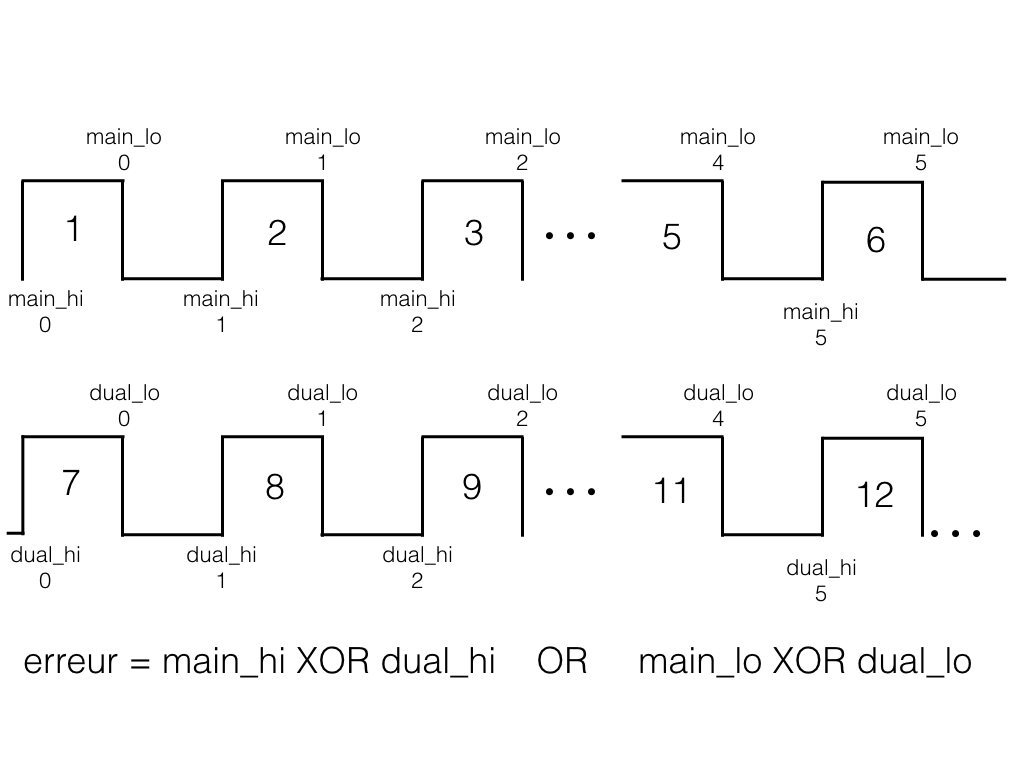
\includegraphics[scale=1.0]{DDR}
%		\caption{Exemple de Double Data Rate}
%		\label{fig:DDR}
%	\end{center}
%\end{figure}

\subsection{Quelles sont les faiblesses de cette sécurité?}

Le problème avec cette façon de sécurisé l'AES est que si l'on change la valeur d'un octet pendant exactement 6 cycles, la valeur du premier calculs sera identique au deuxième calcul.
Ainsi, il ne sera plus possible de faire remonter l'erreur. Cela permettrai à l'attaquant de faire changer un octet d'un

\subsection{Implémentation de l'attaque par faute}

En utilisant la faiblesse expliquée précedement, notre implémentation
consiste à introduire une faute de retournement de bits sur le port
\texttt{in\_hi}, sur 8 bits, de la colonne 0. Nous nous basons sur un
modèle réaliste d'injection de faute où, grâce à un laser, l'attaquant
pourrait retourner les 8 bits de ce port.\\
\texttt{in\_hi\_sig <= in\_hi;\\  lin\_0\_in <= in\_hi\_sig XOR fault\_sig;} \\
Le signal \texttt{fault\_sig} est remonté jusque dans le fichier top, comme un
port du composant \texttt{aes\_core}, pour pouvoir générer l'attaque.
Grâce au XOR,
un bit à 1 dans le signal \texttt{fault\_sig} retournera le bit correspondant
dans le signal \texttt{in\_hi} et créera une faute.
Précisons que nous n'attaquons que la première colonne du DataUnit et que ce
même signal \texttt{fault\_sig} est laissé à \texttt{"00000000"} pour les trois
autres colonnes. \\
Nous avons tout d'abord testé cette implémentation en modifiant le test bench
VHDL qui instancie notre IP. Nous avons rajouté un process \texttt{fault},
qui incrémente un compteur à chaque front montant et qui le remet à zéro à
chaque début de chiffrement. Après un certain nombre de cycles, nous injectons
la faute de retournement de bit (signal \texttt{fault\_sig} à  \texttt{"11111111"}),
pendant exactement 6 cycles afin que les deux registres DDR soient affectés par
l'attaque. \\
En utilisant les données fournies par la publication 197 du FIPS (Federal Information
Processing Standard), c'est à dire le texte d'entrée, la clée et le texte chiffré,
nous pouvons vérifier que notre implémentation fonctionne. Si c'est la cas,
la donnée d'entrée ne doit jamais changer pendant le chiffrement, le signal
de sortie de \texttt{aes\_core}, \texttt{error}, ne doit jamais passer à 1 et
la donnée de sortie doit être différente de la donnée attendue. \\
Nous avons obtenu de tels résultats, voir figure.


% Utilisation du signal fault_sig pour déterminer quels bits
% seront flippés (avec un XOR)
% Utilisation du fichier user_logic pour écrire le code de test

\subsection{Embarcation du code}

% Code en C pour contrôler l'IP à travers les registres, processeur MicroBlaze
% Simulation après synthese sur processeur MicroBlaze non fonctionelle, faute
% détéctée.

\subsection{Conclusion}
